% Provenance (never printed): see sources/outline_sources.md (Year 1: the general
% circulation of the atmosphere, Hadley, Ferrel and polar cells, the ITCZ, Walker cells,
% jet streams, the geostrophic wind, depressions and anticyclones). Exercise and problem
% values in the Book 3 scratch calculator calc/ch28.py; figures from
% figdata/bachelor-1/angular_momentum_wind.py, weather_map.py (an invented map) and
% general_circulation.py (NCEP-NCAR Reanalysis 1, long-term means 1991-2020, datasets
% bachelor-1-ncep-{uwnd-p,vwnd-p,uwnd-sfc,slp,prate-monthly}).
% Physics owns the Coriolis force and the hydrostatic relation (recalled). Book 1 (g8) gave
% the global winds, the convection cell, depressions and anticyclones, isobars and the
% rotation of the wind around them, in words: re-founded here with forces and data.
% ENSO and the monsoons are the Year 2 volume's; the thermal wind the Year 3 volume's.
\chapter{La circulación general de la atmósfera}\label{ch:b1:atmospheric-circulation}

Los veleros que cruzaron desde Europa y África hacia América dependían de los vientos \omterm{def:b1:atmospheric-circulation:winds}{alisios}, los levantes constantes de los trópicos. Más cerca del ecuador, a unos cinco grados de él, esos mismos vientos se apagaban, en el cinturón de calmas y chubascos persistentes que los marineros llamaban las calmas ecuatoriales. Muy por encima de ambos, a unos nueve kilómetros de altura, estrechos ríos de aire llamados \omterm{def:b1:atmospheric-circulation:jet}{corrientes en chorro} pueden soplar a más de \qty{440}{km/h}. Este capítulo explica los tres: por qué el aire que se mueve sobre un planeta en rotación acaba soplando a lo largo de las isobaras y no a través de ellas, cómo el excedente de los trópicos impulsa una gran célula de circulación a cada lado del ecuador, y por qué el aire que sale del ecuador en altura se convierte en un chorro del oeste.
% ledger: nos:trade-winds, nos:doldrums, noaajs:jet

\begin{omfigure}
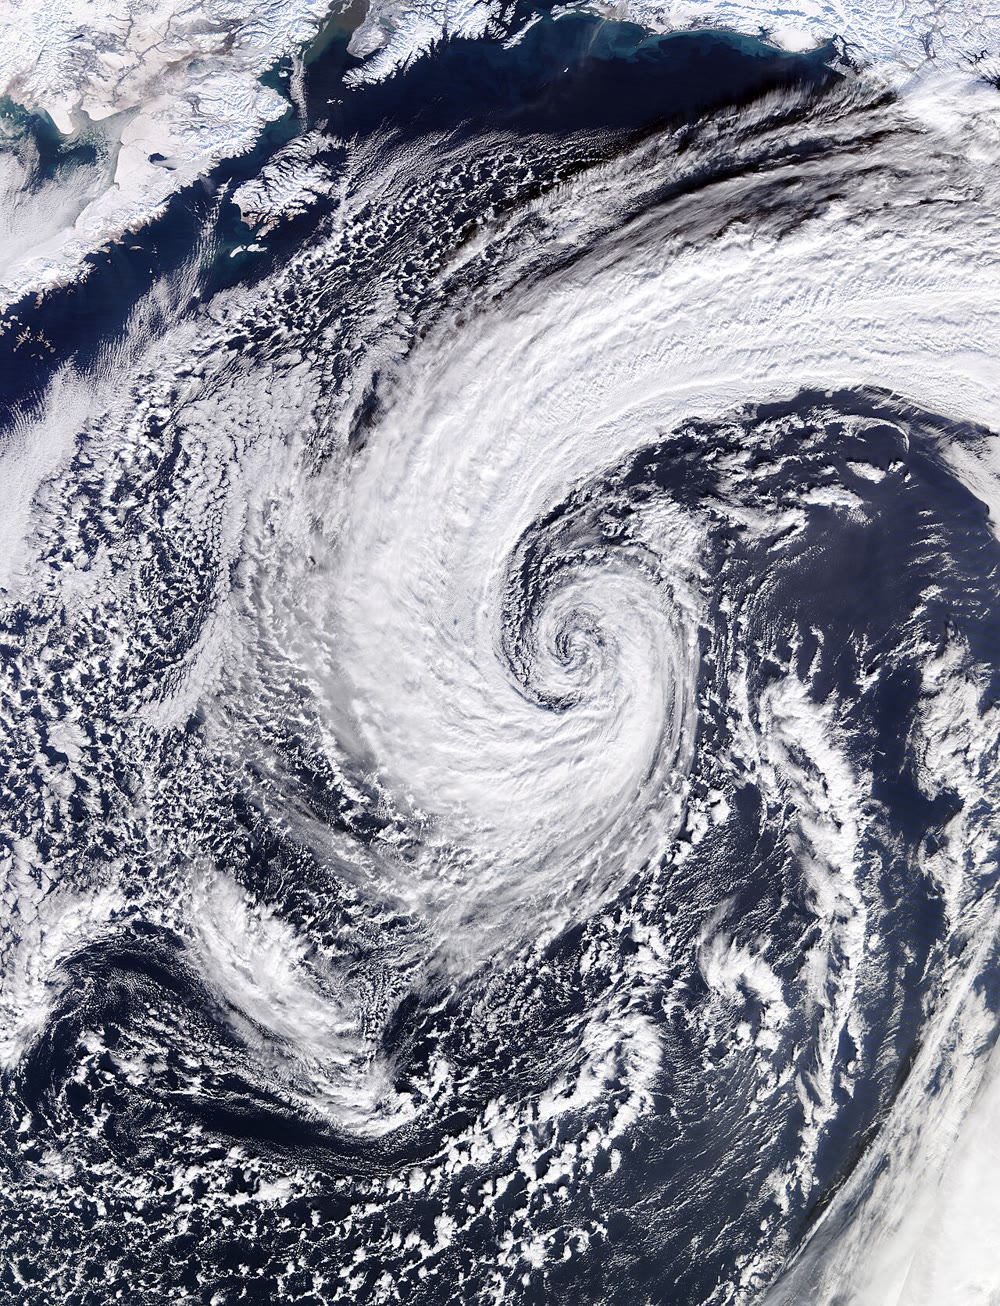
\includegraphics[width=0.5\linewidth]{images/book3/b1-alaska-low.jpg}

{\small Un \omterm{def:b1:atmospheric-circulation:cyclone}{ciclón} extratropical sobre el golfo de Alaska el 28 de enero de 2018, visto por el instrumento MODIS desde órbita; la costa de Alaska, cubierta de nieve, está arriba a la izquierda, y el norte está aproximadamente arriba. Las bandas de nubes se enroscan en sentido antihorario hacia el centro, como lo hace el aire de una depresión del hemisferio norte. (NASA, MODIS/LANCE, dominio público, vía Wikimedia Commons.)}
\label{fig:b1:atmospheric-circulation:alaska}
\end{omfigure}
% ledger: commons:alaska-low, nws:cyclone

\begin{recall}
Los libros de física dan la relación hidrostática y la fuerza de Coriolis: en un
sistema que gira con velocidad angular $\vec\Omega$, un cuerpo de masa $m$ que se mueve
a velocidad $\vec v$ respecto al sistema siente la fuerza ficticia
$-2m\,\vec\Omega\times\vec v$, perpendicular a su movimiento. Para la Tierra,
$\Omega = 2\pi/T_\star$ con el día sidéreo $T_\star = \qty{23.9345}{h}$, es decir,
$\Omega = \qty{7.292e-5}{rad.s^{-1}}$. El libro 1 describió los vientos globales (los \omterm{def:b1:atmospheric-circulation:winds}{alisios}, los \omterm{def:b1:atmospheric-circulation:winds}{vientos del oeste}, los levantes polares), la célula de convección, las depresiones y los \omterm{def:b1:atmospheric-circulation:cyclone}{anticiclones}, las isobaras de un mapa del tiempo y el giro del viento alrededor de los centros. \Cref{ch:b1:fluid-envelopes-structure} dio la \omterm{def:b1:fluid-envelopes-structure:standard-atmosphere}{atmósfera estándar} y el \omterm{def:b1:fluid-envelopes-structure:lapse-rate}{gradiente adiabático seco}, y \cref{ch:b1:radiation-heat-transport} el transporte de calor hacia los polos que lleva la circulación.
% ledger: earth:Trot, nws:coriolis
\end{recall}

\section{Fuerzas sobre el aire en movimiento}\label{sec:b1:atmospheric-circulation:forces}

Una porción de aire es empujada por la presión del aire que la rodea, atraída por la gravedad, frenada por la fricción cerca del suelo y, vista desde la Tierra en rotación, desviada por la fuerza de Coriolis. La gravedad y la fuerza vertical de presión se equilibran casi exactamente: es la relación hidrostática. El tiempo lo hacen las fuerzas que quedan en la horizontal.

\begin{definition}[Fuerza del gradiente de presión]\label{def:b1:atmospheric-circulation:pgf}
La \emph{fuerza del gradiente de presión}\index{fuerza del gradiente de presión} es la fuerza neta que ejerce sobre una porción de fluido la presión del fluido que la rodea. Por unidad de masa es $-(1/\rho)\nabla p$, donde $\rho$ es la densidad y $\nabla p$ el gradiente de presión: apunta de la presión alta a la baja, a través de las isobaras.
\end{definition}
% ledger: nws:geostrophic

\begin{proposition}[La fuerza del gradiente de presión]\label{prop:b1:atmospheric-circulation:pgf}
En una porción de volumen $\mathrm dV$ y densidad $\rho$, la presión del fluido circundante ejerce la fuerza $-\nabla p\,\mathrm dV$, una aceleración $-(1/\rho)\nabla p$.
\end{proposition}

\begin{proof}
Tómese una pequeña caja con aristas $\mathrm dx$, $\mathrm dy$, $\mathrm dz$ a lo largo de los ejes. En su cara en $x$, la presión empuja en la dirección $+x$ con la fuerza
$p(x)\,\mathrm dy\,\mathrm dz$; en su cara en $x + \mathrm dx$, en la dirección $-x$, con $p(x + \mathrm dx)\,\mathrm dy\,\mathrm dz$. La fuerza neta a lo largo de
$x$ es $[p(x) - p(x + \mathrm dx)]\,\mathrm dy\,\mathrm dz = -(\partial p/\partial
x)\,\mathrm dV$, y lo mismo a lo largo de $y$ y $z$. El total es $-\nabla p\,
\mathrm dV$; dividido por la masa $\rho\,\mathrm dV$ da la aceleración.
\end{proof}

Una presión uniforme no ejerce fuerza neta: solo empujan sus diferencias. En un mapa del tiempo el gradiente horizontal se lee en las isobaras: su tamaño es el salto de presión entre dos isobaras dividido por su distancia. Para isobaras separadas \qty{4}{hPa} y \qty{400}{km} al nivel del mar, donde $\rho \approx \qty{1.225}{kg.m^{-3}}$, la
aceleración es $400/(1.225 \times \num{4e5}) = \qty{8.2e-4}{m.s^{-2}}$, menos de una diezmilésima de $g$, pero suficiente para llevar el aire desde el reposo hasta \qty{10}{m/s} en
tres horas y media.
% ledger: ussa76:sea-level

El aire siente la fuerza de Coriolis porque se observa desde la Tierra en rotación. Su parte horizontal depende de la \omterm{def:b1:spherical-astronomy:geographic}{latitud} a través de un solo número.

\begin{definition}[Parámetro de Coriolis]\label{def:b1:atmospheric-circulation:coriolis-parameter}
El \emph{parámetro de Coriolis}\index{parámetro de Coriolis} a la \omterm{def:b1:spherical-astronomy:geographic}{latitud} $\varphi$ es
$f = 2\Omega\sin\varphi$, donde $\Omega$ es la velocidad angular de la Tierra. Es positivo en el hemisferio norte, negativo en el sur, cero en el ecuador, y máximo en los polos, $2\Omega = \qty{1.458e-4}{s^{-1}}$.
\end{definition}
% ledger: earth:Trot

\begin{proposition}[Aceleración horizontal de Coriolis]\label{prop:b1:atmospheric-circulation:coriolis}
Para un viento horizontal $\vec v$ a la \omterm{def:b1:spherical-astronomy:geographic}{latitud} $\varphi$, la parte horizontal de la aceleración de Coriolis es $-f\,\vec k\times\vec v$, donde $\vec k$ es la vertical hacia arriba: tiene tamaño $|f|\,|\vec v|$ y apunta perpendicular al viento, a su derecha en el hemisferio norte y a su izquierda en el sur.
\end{proposition}

\begin{proof}
Úsense ejes locales $x$ hacia el este, $y$ hacia el norte, $z$ hacia arriba. El vector de rotación de la Tierra yace en el plano meridiano, formando
con el horizonte norte el ángulo $\varphi$: $\vec\Omega =
\Omega(0, \cos\varphi, \sin\varphi)$. Para $\vec v = (u, v, 0)$,
\[
  \vec\Omega\times\vec v = \Omega\,(-v\sin\varphi,\ u\sin\varphi,\ -u\cos\varphi),
  \qquad -2\vec\Omega\times\vec v = (f v,\ -f u,\ 2\Omega u\cos\varphi).
\]
Como $\vec k\times\vec v = (-v, u, 0)$, la parte horizontal $(fv, -fu)$ es
$-f\,\vec k\times\vec v$. El vector $\vec k\times\vec v$ es $\vec v$ girado \ang{90} en sentido antihorario visto desde arriba; su opuesto es $\vec v$ girado en sentido horario, a la derecha, cuando $f > 0$, y a la izquierda cuando $f < 0$.
\end{proof}
% ledger: earth:Trot

La parte vertical, $2\Omega u\cos\varphi$, es como mucho \qty{1.5e-3}{m.s^{-2}} para un viento de \qty{10}{m/s}, unas \num{1.5e-4} de $g$: el equilibrio hidrostático la absorbe. La parte horizontal, por pequeña que sea, no tiene rival en la atmósfera libre por encima de la capa de fricción, y en horas da forma a todo viento.

Cerca del suelo, el aire además roza la superficie. En la capa más baja de un kilómetro, la capa de fricción de los meteorólogos, la fricción cambia tanto la rapidez como la dirección del viento; los remolinos turbulentos llevan hacia arriba el arrastre de la superficie, y la fuerza actúa aproximadamente contra el viento y crece con él. Arriba, en la atmósfera libre, la fricción es pequeña.
% ledger: nws:friction-layer

\section{El viento geostrófico}\label{sec:b1:atmospheric-circulation:geostrophic}

\begin{definition}[Equilibrio geostrófico; viento geostrófico]\label{def:b1:atmospheric-circulation:geostrophic}
Un flujo horizontal está en \emph{equilibrio geostrófico}\index{equilibrio geostrófico} cuando su \omterm{def:b1:atmospheric-circulation:pgf}{fuerza del gradiente de presión} y su fuerza de Coriolis se cancelan. El \emph{viento
geostrófico}\index{viento geostrófico} $\vec v_g$ es el viento que logra este equilibrio para un campo de presión dado: $-(1/\rho)\nabla p - f\,\vec k\times\vec v_g = \vec 0$.
\end{definition}
% ledger: nws:geostrophic

\begin{theorem}[El viento geostrófico]\label{thm:b1:atmospheric-circulation:geostrophic}
Lejos del ecuador,
\[
  \vec v_g = \frac{1}{\rho f}\,\vec k\times\nabla p, \qquad
  |\vec v_g| = \frac{|\nabla p|}{\rho\,|f|} .
\]
El \omterm{def:b1:atmospheric-circulation:geostrophic}{viento geostrófico} sopla a lo largo de las isobaras, más deprisa donde están más juntas.
En el hemisferio norte deja la baja presión a su izquierda; en el hemisferio sur, a su derecha.
\end{theorem}

\begin{proof}
Para un vector horizontal $\vec w$, $\vec k\times(\vec k\times\vec w) = -\vec w$.
Aplicando $\vec k\times$ al equilibrio $f\,\vec k\times\vec v_g = -(1/\rho)\nabla p$
se obtiene $-f\vec v_g = -(1/\rho)\,\vec k\times\nabla p$, de donde sale la fórmula, válida donde
$f \neq 0$. Como $\vec k\times\nabla p$ es perpendicular a $\nabla p$, el viento es perpendicular al gradiente, es decir, a lo largo de las isobaras; su tamaño es $|\nabla
p|/(\rho|f|)$. El vector $\vec k\times\nabla p$ es el gradiente girado \ang{90} en sentido antihorario. Mirando a lo largo de él, el gradiente, que apunta a la presión alta, queda a la derecha, así que la baja presión queda a la izquierda; para $f > 0$ el viento tiene la dirección de $\vec k\times\nabla p$, para $f < 0$ la contraria.
\end{proof}

\begin{example}[Un viento leído en las isobaras]\label{ex:b1:atmospheric-circulation:geostrophic}
A \ang{50} N, $f = 2 \times \num{7.292e-5} \times \sin\ang{50} = \qty{1.117e-4}{s^{-1}}$.
Isobaras separadas \qty{4}{hPa} y \qty{400}{km} dan $|\nabla p| = 400/\num{4e5} =
\qty{1.0e-3}{Pa.m^{-1}}$ y, con $\rho = \qty{1.225}{kg.m^{-3}}$, un \omterm{def:b1:atmospheric-circulation:geostrophic}{viento geostrófico} de
$\num{1.0e-3}/(1.225 \times \num{1.117e-4}) = \qty{7.3}{m/s}$. La misma separación a \ang{20} N, donde $f$ es menos de la mitad, daría
\qty{16.4}{m/s}.
\end{example}
% ledger: earth:Trot, ussa76:sea-level

El equilibrio no es instantáneo. El aire puesto en movimiento por un gradiente de presión gira bajo la fuerza de Coriolis a razón de $f$, alrededor de una vez cada $2\pi/f$, unas dieciséis horas a \ang{50}; los patrones que duran más de unas pocas horas y son más grandes que unos cientos de kilómetros se aproximan al \omterm{def:b1:atmospheric-circulation:geostrophic}{equilibrio geostrófico}. Cerca del ecuador $f$ tiende a cero, la fórmula deja de valer, y los vientos del trópico profundo no son geostróficos.

\begin{omfigure}
\begin{tikzpicture}[>={Stealth[length=2.2mm]}, font=\scriptsize]
  % left panel: geostrophic balance
  \begin{scope}
    \draw[isobar] (-2.4,1.2) -- (2.4,1.2) node[right] {\qty{996}{hPa}};
    \draw[isobar] (-2.4,0) -- (2.4,0) node[right] {\qty{1000}{hPa}};
    \draw[isobar] (-2.4,-1.2) -- (2.4,-1.2) node[right] {\qty{1004}{hPa}};
    \node[pressure low] at (0,2.0) {B};
    \node[pressure high] at (0,-2.0) {A};
    \fill (0,0) circle (1.6pt);
    \draw[->, very thick, omThm] (0,0) -- (0,1.0);
    \node[omThm, anchor=east] at (-0.08,0.6) {gradiente de presión};
    \draw[->, very thick, omDef] (0,0) -- (0,-1.0);
    \node[omDef, anchor=east] at (-0.08,-0.6) {Coriolis};
    \draw[->, line width=1.6pt, black] (0,0) -- (1.9,0) node[above, pos=0.75] {viento $\vec v_g$};
    \node[anchor=north] at (0,-2.4) {sin fricción: geostrófico};
  \end{scope}
  % right panel: with friction (alpha = 25 deg, V = Vg cos alpha)
  \begin{scope}[xshift=7.4cm]
    \draw[isobar] (-2.4,1.2) -- (2.4,1.2) node[right] {\qty{996}{hPa}};
    \draw[isobar] (-2.4,0) -- (2.4,0) node[right] {\qty{1000}{hPa}};
    \draw[isobar] (-2.4,-1.2) -- (2.4,-1.2) node[right] {\qty{1004}{hPa}};
    \node[pressure low] at (0,2.0) {B};
    \node[pressure high] at (0,-2.0) {A};
    \fill (0,0) circle (1.6pt);
    \draw[->, very thick, omThm] (0,0) -- (0,1.0);
    \node[omThm, anchor=east] at (-0.08,0.6) {gradiente de presión};
    \draw[->, very thick, omDef] (0,0) -- ({1.0*cos(25)*sin(25)},{-1.0*cos(25)*cos(25)});
    \node[omDef, anchor=west] at (0.42,-0.62) {Coriolis};
    \draw[->, very thick, omMeth] (0,0) -- ({-1.0*sin(25)*cos(25)},{-1.0*sin(25)*sin(25)})
      node[below left, inner sep=1pt] {fricción};
    \draw[->, line width=1.6pt, black] (0,0) -- ({1.9*cos(25)*cos(25)},{1.9*cos(25)*sin(25)})
      node[above, inner sep=2pt] {viento $\vec v$};
    \draw[black!50, dashed] (0,0) -- (1.9,0);
    \draw[black!60] (1.0,0) arc[start angle=0, end angle=25, radius=1.0];
    \node[black!70] at (1.22,0.22) {$\alpha$};
    \node[anchor=north] at (0,-2.4) {con fricción: más lento, a través de las isobaras};
  \end{scope}
\end{tikzpicture}

{\small Fuerzas sobre una porción de aire en el hemisferio norte, con baja presión al norte. Izquierda: en la atmósfera libre la \omterm{def:b1:atmospheric-circulation:pgf}{fuerza del gradiente de presión} (rojo) y la fuerza de Coriolis (azul) se cancelan, y el viento sopla a lo largo de las isobaras con la baja a su izquierda. Derecha: cerca del suelo la fricción (verde) actúa contra el viento; las tres fuerzas se equilibran solo si el viento es más lento y está girado un ángulo $\alpha$ hacia la baja (dibujado para $\alpha = \ang{25}$ y el arrastre de \cref{prop:b1:atmospheric-circulation:friction}).}
\label{fig:b1:atmospheric-circulation:balance}
\end{omfigure}

\begin{proposition}[La fricción gira el viento hacia la baja presión]\label{prop:b1:atmospheric-circulation:friction}
Supóngase que un viento horizontal estacionario $\vec v$ está sometido a la \omterm{def:b1:atmospheric-circulation:pgf}{fuerza del gradiente de presión}, a la fuerza de Coriolis y a una fuerza de fricción $-\vec v/\tau$, con $\tau > 0$, a una \omterm{def:b1:spherical-astronomy:geographic}{latitud} donde $f > 0$. Entonces el viento cruza las isobaras hacia la baja presión con el ángulo $\alpha$, donde $\tan\alpha = 1/(f\tau)$, y su rapidez es $|\vec v| =
|\vec v_g|\cos\alpha$, menor que el \omterm{def:b1:atmospheric-circulation:geostrophic}{viento geostrófico}.
\end{proposition}

\begin{proof}
Sea $V = |\vec v|$, $\hat v$ el vector unitario a lo largo del viento y $\hat n$ el vector unitario perpendicular a él, a su izquierda. El equilibrio es $-(1/\rho)\nabla p - f\,
\vec k\times\vec v - \vec v/\tau = \vec 0$, y $\vec k\times\vec v = V\hat n$.
A lo largo de $\hat v$: $-(1/\rho)\,\nabla p\cdot\hat v = V/\tau > 0$, así que el viento tiene una componente hacia abajo del gradiente de presión, hacia la baja presión. A lo largo de $\hat n$:
$-(1/\rho)\,\nabla p\cdot\hat n = fV$. La \omterm{def:b1:atmospheric-circulation:pgf}{fuerza del gradiente de presión}, de tamaño $P =
|\nabla p|/\rho = f|\vec v_g|$, tiene por tanto componentes $V/\tau$ a lo largo del viento y
$fV$ a través de él: forma con el viento el ángulo $\beta$ con $\tan\beta =
1/(f\tau)$, y $P^2 = V^2(f^2 + 1/\tau^2)$. Las isobaras son perpendiculares al
gradiente, así que el viento las cruza con $\alpha = \beta$, y $V = P/\sqrt{f^2 +
1/\tau^2} = (P/f)\cos\alpha = |\vec v_g|\cos\alpha$.
\end{proof}

Una superficie más rugosa significa un arrastre más fuerte, un $\tau$ más corto y un ángulo mayor: el viento cruza las isobaras más empinadamente sobre tierra que sobre el mar. La fricción real no es exactamente lineal en el viento, pero la conclusión, más lenta y girada hacia la baja, es general.

\begin{remark}[El viento de gradiente]\label{rem:b1:atmospheric-circulation:gradient}
Alrededor de un centro las isobaras están curvadas, y el aire que las sigue se acelera hacia el centro de curvatura, $V^2/r$ para un círculo de radio $r$. Alrededor de una baja en el hemisferio norte, la \omterm{def:b1:atmospheric-circulation:pgf}{fuerza del gradiente de presión} debe superar entonces a la de Coriolis: $fV + V^2/r = f|\vec v_g|$, y el viento, llamado viento de gradiente, es más débil que el geostrófico. Alrededor de un alto, la fuerza de Coriolis debe superar a la del gradiente de presión, $fV - V^2/r = f|\vec v_g|$: el viento es más fuerte, pero la ecuación tiene solución solo si $|\vec v_g| \leq fr/4$, lo que prohíbe gradientes de presión fuertes cerca del centro de un \omterm{def:b1:atmospheric-circulation:cyclone}{anticiclón} (\cref{exo:b1:atmospheric-circulation:10}).
\end{remark}

\section{Depresiones y anticiclones}\label{sec:b1:atmospheric-circulation:cyclones}

\begin{definition}[Ciclón, anticiclón]\label{def:b1:atmospheric-circulation:cyclone}
Un \emph{ciclón}\index{ciclón} es una circulación de gran escala de vientos alrededor de un centro de baja presión, una depresión; un \emph{anticiclón}\index{anticiclón} es una circulación alrededor de un centro de alta presión. Un ciclón gira en sentido antihorario en el hemisferio norte y en sentido horario en el sur; un anticiclón al revés.
\end{definition}
% ledger: nws:cyclone

Los sentidos de giro se siguen de \cref{thm:b1:atmospheric-circulation:geostrophic}: en el hemisferio norte, un viento que deja la baja a su izquierda da la vuelta a la baja en sentido antihorario y a un alto en sentido horario. Vistas desde el espacio, las nubes de una depresión trazan el giro (la fotografía al principio del capítulo); en el hemisferio sur las espirales son imágenes especulares.
% ledger: nws:cyclone, commons:alaska-low

\begin{history}[La ley de Buys Ballot, 1857]
En 1857 el meteorólogo neerlandés C.~H.~D. Buys Ballot enunció una regla hallada en las observaciones: en el hemisferio norte, una persona de espaldas al viento tiene la baja presión a la izquierda y la alta a la derecha; en el hemisferio sur, lo contrario. No sabía que el meteorólogo estadounidense William Ferrel ya la había deducido de la teoría, y más tarde reconoció la prioridad de Ferrel.
El \omterm{def:b1:atmospheric-circulation:geostrophic}{viento geostrófico} es la ley en ecuaciones.
\end{history}
% ledger: skybrary:buys-ballot

La fricción añade un giro importante. Cerca del suelo el viento cruza las isobaras hacia la baja presión (\cref{prop:b1:atmospheric-circulation:friction}): alrededor de una depresión el aire se enrolla hacia dentro, converge cerca del suelo y debe elevarse. El aire que sube se expande y se enfría al ritmo del \omterm{def:b1:fluid-envelopes-structure:lapse-rate}{gradiente adiabático seco} (\cref{ch:b1:fluid-envelopes-structure}), y una vez saturado su vapor de agua se condensa: las depresiones traen nubes y lluvia. Alrededor de un \omterm{def:b1:atmospheric-circulation:cyclone}{anticiclón} el aire del suelo se enrolla hacia fuera; desciende aire desde arriba para reemplazarlo, se calienta por compresión, y sus nubes se evaporan: los \omterm{def:b1:atmospheric-circulation:cyclone}{anticiclones} traen tiempo estable, a menudo despejado.
% ledger: nws:dalr

El mapa de abajo es un ejemplo inventado, calculado y no observado: una depresión de \qty{28}{hPa} de profundidad y un \omterm{def:b1:atmospheric-circulation:cyclone}{anticiclón} de \qty{20}{hPa} de altura sobre un fondo de \qty{1013}{hPa}, centrados cerca de \ang{50} N. En cada estación la plumilla de viento muestra el \omterm{def:b1:atmospheric-circulation:geostrophic}{viento geostrófico} calculado a partir del mapa con \cref{thm:b1:atmospheric-circulation:geostrophic}.

\begin{omfigure}
\pgfplotstableread{figdata/out/bachelor-1-weather_map-stations.dat}\wmstations
\pgfplotstableread{figdata/out/bachelor-1-weather_map-labels.dat}\wmlabels
\begin{tikzpicture}
\begin{axis}[x=0.0038cm, y=0.0038cm, disabledatascaling, anchor=origin,
  xmin=-1800, xmax=1800, ymin=-1200, ymax=1200, xtick=\empty, ytick=\empty,
  axis background/.style={fill=blue!4}, clip=true]
% figdata/bachelor-1/weather_map.py (invented pressure field); ledger: earth:Trot, ussa76:sea-level
\addplot[isobar, unbounded coords=jump] table[x=x, y=y] {figdata/out/bachelor-1-weather_map-isobars.dat};
\addplot[black!45, dashed, domain=-1800:1800] {0};
\addplot[only marks, mark=none, nodes near coords, point meta=explicit symbolic,
  nodes near coords style={font=\tiny, fill=blue!4, inner sep=0.5pt, anchor=center}]
  table[x=x, y=y, meta=p] {\wmlabels};
\node[pressure low] at (axis cs:-500,150) {B};
\node[pressure high] at (axis cs:1050,-250) {A};
\node[font=\tiny, anchor=south west, black!60] at (axis cs:-1790,5) {\ang{50} N};
\end{axis}
\pgfplotstablegetrowsof{\wmstations}
\pgfmathtruncatemacro{\wmlast}{\pgfplotsretval-1}
\begin{scope}
\clip (-6.84,-4.56) rectangle (6.84,4.56);
\foreach \i in {0,...,\wmlast}{
  \pgfplotstablegetelem{\i}{x}\of\wmstations \let\wx\pgfplotsretval
  \pgfplotstablegetelem{\i}{y}\of\wmstations \let\wy\pgfplotsretval
  \pgfplotstablegetelem{\i}{speed_kn}\of\wmstations \let\ws\pgfplotsretval
  \pgfplotstablegetelem{\i}{from_deg}\of\wmstations \let\wd\pgfplotsretval
  \pic[transform shape] at ({\wx*0.0038},{\wy*0.0038}) {windbarb={\ws}{\wd}};
}
\end{scope}
\pic[transform shape] at (-6.5,-4.0) {scalebar={1.9}{\qty{500}{km}}};
\pic[scale=0.7, transform shape] at (-6.45,3.2) {northarrow};
\end{tikzpicture}

{\small Un mapa inventado de presión a nivel del mar cerca de \ang{50} N (isobaras cada \qty{4}{hPa}; presiones centrales \qty{986}{hPa} y \qty{1033}{hPa}). Cada plumilla apunta hacia el \omterm{def:b1:atmospheric-circulation:geostrophic}{viento geostrófico} de su estación, con el asta hacia de donde viene el viento; una pluma entera es \qty{10}{kn}, media pluma \qty{5}{kn}, un banderín \qty{50}{kn} (\qty{1}{kn} = \qty{0.514}{m/s}). Los vientos giran en sentido antihorario alrededor de la baja y en sentido horario alrededor de la alta, y son más fuertes donde las isobaras se agolpan entre las dos, alcanzando \qty{36}{m/s}.}
\label{fig:b1:atmospheric-circulation:weather-map}
\end{omfigure}
% ledger: earth:Trot, ussa76:sea-level (computed in figdata/bachelor-1/weather_map.py)

\section{La circulación de tres células}\label{sec:b1:atmospheric-circulation:cells}

Promediados alrededor del globo y a lo largo de muchos años, los vientos que soplan hacia el norte o el sur son débiles, de unos metros por segundo como mucho, pero transportan mucho aire. Su patrón se ve mejor en la masa que fluye entre el ecuador y los polos.

\begin{definition}[Función de corriente meridional media]\label{def:b1:atmospheric-circulation:streamfunction}
La \emph{función de corriente meridional media}\index{función de corriente meridional media} $\psi(p, \varphi)$ es la \omterm{def:b1:observing-the-sky:extinction}{masa de aire} por segundo que cruza la \omterm{def:b1:spherical-astronomy:geographic}{latitud}
$\varphi$ hacia el norte por encima del nivel de presión $p$, en la media zonal y temporal:
\[
  \psi(p, \varphi) = \frac{2\pi a_\oplus\cos\varphi}{g}\int_0^p [v]\,\mathrm dp' ,
\]
donde $[v]$ es el viento hacia el norte promediado alrededor del paralelo. Se mide en
\unit{kg.s^{-1}}.
\end{definition}

Como $\mathrm dp' = -\rho g\,\mathrm dz$ por la relación hidrostática, $2\pi a_\oplus
\cos\varphi\,[v]\,\mathrm dp'/g$ es el flujo de masa a través de un anillo del paralelo. El aire que cruza el paralelo por encima de $p$ debe cruzarlo en sentido contrario por debajo de $p$, pues la masa no se acumula: $\psi$ se anula en el suelo y en el tope, y sus líneas de igual valor son las trayectorias de la circulación media. Una célula con $\psi > 0$ gira en sentido horario cuando se dibuja con el Polo Norte a la derecha: hacia el norte por encima, hacia el sur por debajo.

\begin{omfigure}
\begin{tikzpicture}
\begin{groupplot}[group style={group size=1 by 2, vertical sep=1.3cm},
  width=0.82\linewidth, height=4.6cm, view={0}{90}, xmin=-70, xmax=70, ymin=100,
  ymax=1000, y dir=reverse, ytick={200,400,600,800,1000}, xtick={-60,-40,...,60},
  tick label style={font=\scriptsize}, label style={font=\small},
  ylabel={presión (\unit{hPa})},
  colormap={omdiv}{rgb255=(33,102,172) rgb255=(146,197,222) rgb255=(247,247,247)
    rgb255=(244,165,130) rgb255=(178,24,43)},
  point meta min=-22, point meta max=22, colorbar,
  colorbar style={width=0.25cm, y dir=normal, ytick={-20,-10,0,10,20}, tick label style={font=\scriptsize},
    ylabel={$\psi$ (\qty{e10}{kg.s^{-1}})}, ylabel style={font=\scriptsize}},
  axis on top, grid=none]
\nextgroupplot[title={diciembre--febrero}, title style={font=\small}]
% figdata/bachelor-1/general_circulation.py; ledger: data:b3-ncep-circ, psl:ncep-r1
\addplot3[surf, shader=interp, mesh/ordering=x varies, mesh/cols=73]
  table[x=lat, y=p, z=psi] {figdata/out/bachelor-1-general_circulation-psi-djf.dat};
\addplot3[black, line width=0.5pt, unbounded coords=jump]
  table[x=lat, y=p, z expr=40] {figdata/out/bachelor-1-general_circulation-psi0-djf.dat};
\nextgroupplot[title={junio--agosto}, title style={font=\small}, xlabel={latitud (\unit{\degree})}]
\addplot3[surf, shader=interp, mesh/ordering=x varies, mesh/cols=73]
  table[x=lat, y=p, z=psi] {figdata/out/bachelor-1-general_circulation-psi-jja.dat};
\addplot3[black, line width=0.5pt, unbounded coords=jump]
  table[x=lat, y=p, z expr=40] {figdata/out/bachelor-1-general_circulation-psi0-jja.dat};
\end{groupplot}
\end{tikzpicture}

{\small La \omterm{def:b1:atmospheric-circulation:streamfunction}{función de corriente meridional media} en el invierno boreal (arriba) y el verano boreal (abajo), a partir del viento zonal medio hacia el norte del NCEP-NCAR Reanalysis~1, medias de 1991--2020 (datos proporcionados por NOAA PSL). Rojo: células en sentido horario en esta vista (ascendiendo en su lado sur), azul: en sentido antihorario; negro: las líneas nulas que separan las células. La \omterm{def:b1:atmospheric-circulation:cells}{célula de Hadley} de invierno cruza el ecuador y empequeñece a la de verano.}
\label{fig:b1:atmospheric-circulation:psi}
\end{omfigure}
% ledger: data:b3-ncep-circ, psl:ncep-r1 (computed in figdata/bachelor-1/general_circulation.py)

En la media anual el reanálisis muestra dos células fuertes a ambos lados del ecuador, con máximos de \qty{8.7e10}{kg/s} cerca de \ang{15} N y \ang{15} S a \qty{400}{hPa}; a \qty{500}{hPa} sus bordes hacia el polo yacen en \ang{33} N y \ang{32} S. Más allá de ellas, dos células más débiles giran en sentido contrario, hasta unos \ang{61} N y \ang{64} S.
Las estaciones remodelan el cuadro: de diciembre a febrero, el invierno boreal, la célula que asciende al sur del ecuador y desciende en los subtrópicos del norte transporta \qty{21.4e10}{kg/s} y llega desde \ang{13} S hasta \ang{31} N; de junio a agosto su imagen especular transporta \qty{18.9e10}{kg/s} desde \ang{17} N hasta \ang{29} S.
% ledger: data:b3-ncep-circ (computed in figdata/bachelor-1/general_circulation.py)

\begin{definition}[Células de Hadley, Ferrel y polares; altas subtropicales]\label{def:b1:atmospheric-circulation:cells}
La circulación meridional media de cada hemisferio tiene tres células. La \emph{célula de Hadley}\index{célula de Hadley} asciende cerca del ecuador, fluye hacia el polo en altura, desciende cerca de \ang{30} y regresa hacia el ecuador en superficie. La \emph{célula de Ferrel}\index{célula de Ferrel}, entre aproximadamente \ang{30} y \ang{60}, gira en sentido contrario: desciende cerca de \ang{30} y asciende cerca de \ang{60}, con su flujo de superficie hacia el polo. La \emph{célula polar}\index{célula polar}, la más pequeña y débil, asciende cerca de \ang{60}, desciende sobre el polo y regresa hacia \ang{60} en superficie. Las \emph{altas subtropicales}\index{alta subtropical} son los cinturones de alta presión a nivel del mar cerca de \ang{30} N y S, bajo las ramas descendentes de las células de Hadley.
\end{definition}
% ledger: noaajs:cells, nws:ferrel-cell, nws:winds

\begin{definition}[Alisios, vientos del oeste]\label{def:b1:atmospheric-circulation:winds}
Los \emph{alisios}\index{alisios} son los vientos superficiales persistentes que soplan desde las \omterm{def:b1:atmospheric-circulation:cells}{altas subtropicales} hacia la baja ecuatorial, desviados por la fuerza de Coriolis hacia el noreste en el hemisferio norte y hacia el sureste en el sur. Los \emph{vientos del oeste}\index{vientos del oeste} son los vientos dominantes desde el oeste de las \omterm{def:b1:spherical-astronomy:geographic}{latitudes} medias, entre unos \ang{35} y \ang{60}. Más allá hacia el polo soplan los levantes polares.
\end{definition}
% ledger: nws:winds, noaajs:cells

La rama superficial de cada célula explica su viento. El flujo de retorno de la \omterm{def:b1:atmospheric-circulation:cells}{célula de Hadley} se dirige hacia el ecuador y la fuerza de Coriolis lo gira hacia el oeste: los \omterm{def:b1:atmospheric-circulation:winds}{alisios}. El flujo superficial de la \omterm{def:b1:atmospheric-circulation:cells}{célula de Ferrel} se dirige hacia el polo y es girado hacia el este: los \omterm{def:b1:atmospheric-circulation:winds}{vientos del oeste}. En la media anual del reanálisis, el viento zonal justo encima del suelo es de \qty{-3.5}{m/s} a \ang{15} N y \qty{-4.4}{m/s} a \ang{15} S (negativo: desde el este), \qty{+1.9}{m/s} a \ang{45} N y \qty{+6.5}{m/s} a \ang{45} S; la presión a nivel del mar alcanza su máximo, \qty{1017.5}{hPa}, cerca de \ang{35} N y \qty{1018.7}{hPa} cerca de \ang{32} S, y baja a \qty{988}{hPa} a \ang{60} S, la profunda vaguada del océano Austral.
% ledger: data:b3-ncep-circ (computed in figdata/bachelor-1/general_circulation.py)

\begin{omfigure}
\begin{tikzpicture}[>={Stealth[length=1.8mm]}, font=\scriptsize]
  % left: the globe with the surface winds
  \def\R{2.6}
  \fill[blue!7] (0,0) circle (\R);
  \draw (0,0) circle (\R);
  \foreach \l in {-60,-30,30,60} {
    \pgfmathsetmacro{\y}{\R*sin(\l)}\pgfmathsetmacro{\x}{\R*cos(\l)}
    \draw[black!45, dashed] (-\x,\y) -- (\x,\y);}
  \draw[black!60] (-\R,0) -- (\R,0);
  \foreach \s in {1,-1} {
    \foreach \x in {-1.7,-0.7,0.3} {
      \draw[->, omThm, line width=0.9pt] (\x+0.3,\s*0.95) -- (\x-0.3,\s*0.45);}
    \foreach \x in {-1.0,0.2} {
      \draw[->, omDef, line width=0.9pt] (\x-0.3,\s*1.45) -- (\x+0.3,\s*1.9);}
    \draw[->, omMeth, line width=0.9pt] (0.25,\s*2.45) -- (-0.25,\s*2.2);
  }
  \node[fill=blue!7, inner sep=1pt, anchor=west] at (0.95,0.72) {alisios del NE};
  \node[fill=blue!7, inner sep=1pt, anchor=west] at (0.95,-0.72) {alisios del SE};
  \node[fill=blue!7, inner sep=1pt, anchor=west] at (0.55,1.72) {vientos del oeste};
  \node[fill=blue!7, inner sep=1pt, anchor=west] at (0.55,-1.72) {vientos del oeste};
  \node[anchor=south] at (0,\R+0.02) {levantes polares};
  \node[anchor=north] at (0,-\R-0.02) {levantes polares};
  \node[anchor=east, align=right] at (-\R-0.05,0) {baja ecuatorial\\(ZCIT)};
  \node[anchor=east, align=right] at ({-\R*cos(30)-0.05},{\R*sin(30)}) {alta subtropical};
  \node[anchor=east, align=right] at ({-\R*cos(30)-0.05},{-\R*sin(30)}) {alta subtropical};
  \node[anchor=east] at ({-\R*cos(60)-0.05},{\R*sin(60)}) {baja subpolar};
  \node[anchor=east] at ({-\R*cos(60)-0.05},{-\R*sin(60)}) {baja subpolar};
  % right: meridional section of the Northern Hemisphere
  \begin{scope}[xshift=4.3cm, yshift=-1.4cm]
    \draw[->] (0,0) -- (6.3,0);
    \foreach \l/\t in {0/\ang{0},2/\ang{30} N,4/\ang{60} N,6/\ang{90} N}
      \draw (\l,0.06) -- (\l,-0.06) node[below] {\t};
    \draw[black!45, dashed] (0,2.6) .. controls (2.4,2.6) and (2.8,1.9) .. (6,1.7)
      node[above left, black!60] {tropopausa};
    \def\cellcw#1#2#3#4{\draw[line width=0.9pt, omThm, postaction=decorate,
      decoration={markings, mark=at position 0.25 with {\arrow{Stealth[length=2mm]}},
      mark=at position 0.75 with {\arrow{Stealth[length=2mm]}}}]
      (#1+#3,#2) arc[start angle=0, end angle=-360, x radius=#3, y radius=#4];}
    \def\cellccw#1#2#3#4{\draw[line width=0.9pt, omDef, postaction=decorate,
      decoration={markings, mark=at position 0.25 with {\arrow{Stealth[length=2mm]}},
      mark=at position 0.75 with {\arrow{Stealth[length=2mm]}}}]
      (#1+#3,#2) arc[start angle=0, end angle=360, x radius=#3, y radius=#4];}
    \cellcw{1}{1.25}{0.85}{1.05}
    \cellccw{3}{1.0}{0.85}{0.75}
    \cellcw{5}{0.85}{0.85}{0.6}
    \node at (1,1.25) {Hadley};
    \node at (3,1.0) {Ferrel};
    \node at (5,0.85) {polar};
  \end{scope}
\end{tikzpicture}

{\small Izquierda: los vientos superficiales de la circulación de tres células, girados a la derecha de su movimiento en el hemisferio norte y a la izquierda en el sur, entre los cinturones de presión. Derecha: las tres células del hemisferio norte en una sección meridiana (altura no a escala); el hemisferio sur es la imagen especular. Los \omterm{def:b1:atmospheric-circulation:winds}{alisios} son la rama de retorno de la \omterm{def:b1:atmospheric-circulation:cells}{célula de Hadley}, los \omterm{def:b1:atmospheric-circulation:winds}{vientos del oeste} la rama superficial de la \omterm{def:b1:atmospheric-circulation:cells}{célula de Ferrel}.}
\label{fig:b1:atmospheric-circulation:three-cells}
\end{omfigure}
% ledger: noaajs:cells, nws:winds, nws:ferrel-cell

\begin{history}[Hadley 1735, Ferrel 1856]
En 1735 George Hadley publicó en las \emph{Philosophical Transactions} un breve artículo sobre la causa de los \omterm{def:b1:atmospheric-circulation:winds}{alisios} generales. Para explicarlos propuso una sola circulación en cada hemisferio, desde el ecuador hasta el polo.
En 1856 William Ferrel publicó \emph{An essay on the winds and currents of the ocean}, en el que el aire de las \omterm{def:b1:spherical-astronomy:geographic}{latitudes} medias fluye hacia el polo y hacia el este cerca de la superficie: la primera descripción de los \omterm{def:b1:atmospheric-circulation:winds}{vientos del oeste} entre \ang{35} y \ang{60}. Su artículo no daba justificación matemática; la circulación que describió es la célula que lleva su nombre.
\end{history}
% ledger: hadley:1735, noaajs:cells, mactutor:ferrel

¿Por qué la \omterm{def:b1:atmospheric-circulation:cells}{célula de Hadley} se detiene cerca de \ang{30} en lugar de llegar al polo, como pensaba Hadley? La respuesta está en el momento angular que el aire lleva respecto al eje de la Tierra.

\begin{proposition}[El viento del momento angular]\label{prop:b1:atmospheric-circulation:angular-momentum}
Un anillo de aire a la \omterm{def:b1:spherical-astronomy:geographic}{latitud} $\varphi$, con viento hacia el este $u$ respecto al suelo,
tiene el momento angular absoluto por unidad de masa respecto al eje de la Tierra $M =
(\Omega a_\oplus\cos\varphi + u)\,a_\oplus\cos\varphi$. Si un anillo en reposo a la \omterm{def:b1:spherical-astronomy:geographic}{latitud}
$\varphi_0$ se desplaza hasta $\varphi$ sin par que actúe sobre él, llega con el viento
\[
  u(\varphi) = \Omega a_\oplus\,\frac{\cos^2\varphi_0 - \cos^2\varphi}{\cos\varphi},
  \qquad\text{y desde el ecuador}\qquad
  u(\varphi) = \Omega a_\oplus\,\frac{\sin^2\varphi}{\cos\varphi} .
\]
\end{proposition}

\begin{proof}
Un anillo a la \omterm{def:b1:spherical-astronomy:geographic}{latitud} $\varphi$ está a la distancia $r = a_\oplus\cos\varphi$ del eje. Su rapidez hacia el este absoluta es la del suelo, $\Omega r$, más el viento
$u$; su momento angular por unidad de masa es $M = (\Omega r + u)\,r$. Sin par, $M$ se conserva: $(\Omega a_\oplus\cos\varphi + u)\cos\varphi = \Omega a_\oplus
\cos^2\varphi_0$, de donde sale la primera fórmula; $\varphi_0 = 0$ da la segunda, pues $1 - \cos^2\varphi = \sin^2\varphi$.
\end{proof}
% ledger: earth:Trot, earth:Rmean

El suelo en el ecuador se mueve hacia el este a $\Omega a_\oplus = \qty{464.6}{m/s}$. El aire que lo deja en reposo en altura y se dirige hacia el polo se acerca al eje y, como un patinador que recoge los brazos, gira más deprisa que el suelo debajo: a \ang{20} soplaría desde el oeste a \qty{58}{m/s}, a \ang{30} a \qty{134}{m/s}, a \ang{40} a \qty{251}{m/s}. No se observa ningún viento de esa fuerza. El viento zonal medio a \qty{200}{hPa} alcanza su máximo, \qty{42.3}{m/s}, cerca de \ang{30} N en el invierno boreal y \qty{40.4}{m/s} cerca de \ang{30} S en el invierno austral.
% ledger: earth:Trot, earth:Rmean, data:b3-ncep-circ (computed in figdata/bachelor-1/angular_momentum_wind.py and general_circulation.py)

\begin{omfigure}
\begin{tikzpicture}
\begin{axis}[omrecord, width=0.78\linewidth, height=6cm, xmin=0, xmax=60, ymin=-25, ymax=150,
  xlabel={latitud (\unit{\degree} N)}, ylabel={viento hacia el este (\unit{m/s})},
  xtick={0,10,...,60}, ytick={0,25,...,150}]
% figdata/bachelor-1/angular_momentum_wind.py, general_circulation.py; ledger: earth:Trot, earth:Rmean, data:b3-ncep-circ
\addplot[black!40, domain=0:60] {0};
\addplot[omThm, line width=1.1pt, restrict y to domain=-10:160] table[x=lat, y=u] {figdata/out/bachelor-1-angular_momentum_wind-curve.dat};
\addplot[black, line width=1.1pt] table[x=lat, y=u] {figdata/out/bachelor-1-general_circulation-u200-djf.dat};
\addplot[black, dashed, line width=0.9pt] table[x=lat, y=u] {figdata/out/bachelor-1-general_circulation-u200-jja.dat};
\node[font=\scriptsize, text=omThm, anchor=west] at (axis cs:31.5,128) {anillo desde el ecuador};
\node[font=\scriptsize, anchor=south] at (axis cs:30,44) {diciembre--febrero};
\node[font=\scriptsize, anchor=north west] at (axis cs:46,-3) {junio--agosto};
\end{axis}
\end{tikzpicture}

{\small El viento hacia el este de un anillo de aire que deja el ecuador en reposo y conserva su momento angular (rojo, \cref{prop:b1:atmospheric-circulation:angular-momentum}), frente al viento zonal medio a \qty{200}{hPa} del reanálisis (negro: invierno boreal; discontinua: verano boreal), NCEP-NCAR Reanalysis~1, medias de 1991--2020, datos proporcionados por NOAA PSL. Ambos concuerdan cerca del ecuador; hacia el polo, desde \ang{15}, el anillo supera cada vez más al viento real.}
\label{fig:b1:atmospheric-circulation:angular-momentum}
\end{omfigure}
% ledger: data:b3-ncep-circ, earth:Trot, earth:Rmean

La proposición da al ramo superior de la \omterm{def:b1:atmospheric-circulation:cells}{célula de Hadley} un límite. A medida que su aire se mueve hacia el polo, su viento del oeste crece, y también la fuerza de Coriolis que lo devuelve hacia el ecuador; mucho antes de alcanzar las velocidades del anillo, el flujo se vuelve inestable y se rompe en grandes remolinos, las depresiones y los \omterm{def:b1:atmospheric-circulation:cyclone}{anticiclones} de las \omterm{def:b1:spherical-astronomy:geographic}{latitudes} medias. Estos remolinos, más que una circulación suave, llevan calor y momento angular hacia el polo más allá de los subtrópicos; la \omterm{def:b1:atmospheric-circulation:cells}{célula de Ferrel} es la firma promediada de su movimiento, y la corriente real es más lenta que el anillo porque los remolinos le quitan parte de su momento angular. Por qué la célula termina cerca de \ang{30} y no en \ang{20} o \ang{40} requiere la teoría de estas inestabilidades, más allá de este volumen.

\begin{dated}{2021}
% ledger: ipcc:hadley-widening
El informe de evaluación del IPCC publicado en 2021 encuentra un \emph{probable} ensanchamiento de la circulación de Hadley desde los años ochenta, sobre todo por su extensión en el hemisferio norte, aunque con solo \emph{confianza media} en la magnitud de los cambios, junto con un fortalecimiento, particularmente en el hemisferio norte (\emph{confianza media}).
\end{dated}

\section{La ZCIT y la circulación de Walker}\label{sec:b1:atmospheric-circulation:itcz}

\begin{definition}[Zona de convergencia intertropical]\label{def:b1:atmospheric-circulation:itcz}
La \emph{zona de convergencia intertropical}\index{zona de convergencia intertropical} (ZCIT) es el cinturón cerca del ecuador donde convergen los \omterm{def:b1:atmospheric-circulation:winds}{alisios} del noreste y del sureste, formando una banda a menudo continua de nubes y tormentas. Es la rama ascendente de las dos \omterm{def:b1:atmospheric-circulation:cells}{células de Hadley}; los vientos ligeros de su superficie son las calmas ecuatoriales de los marineros.
\end{definition}
% ledger: nws:winds, nos:doldrums

\begin{omfigure}
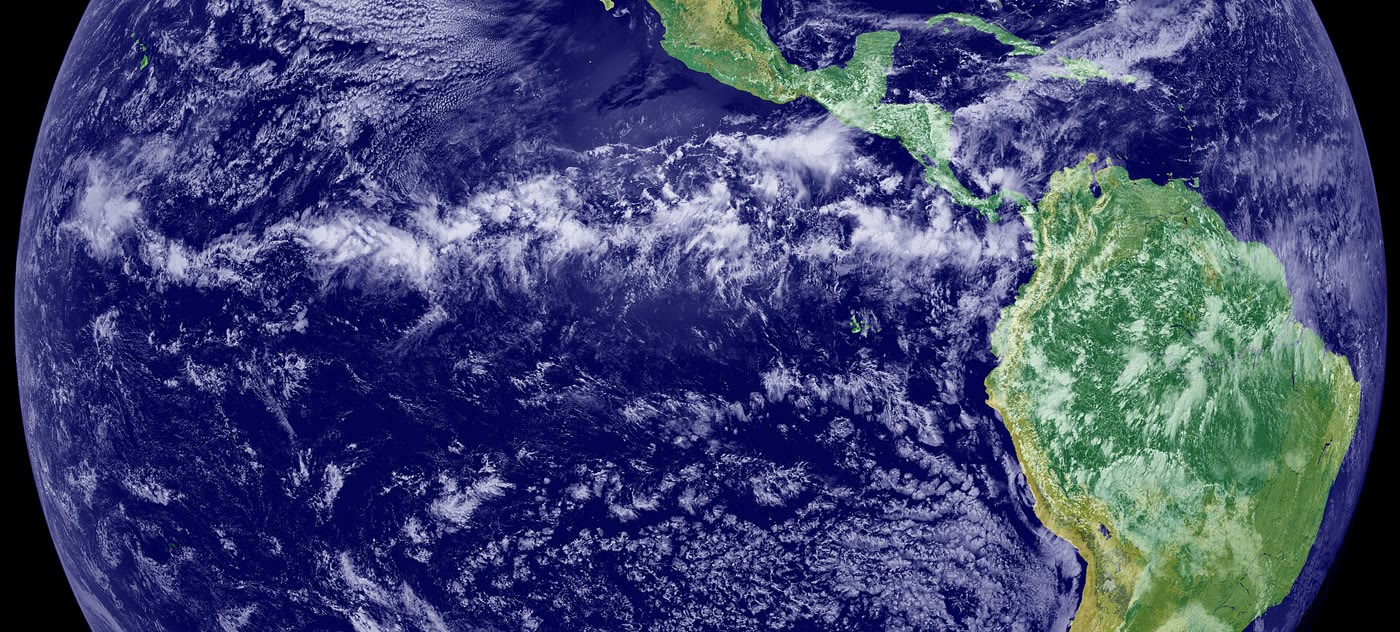
\includegraphics[width=0.8\linewidth]{images/book3/b1-itcz-goes.jpg}

{\small La \omterm{def:b1:atmospheric-circulation:itcz}{zona de convergencia intertropical} sobre el Pacífico oriental: una línea de nubes brillantes que cruza el océano al norte del ecuador, con Centroamérica y Sudamérica a la derecha. La imagen combina datos de nubes del satélite geoestacionario GOES-11 con colores de la cubierta terrestre. (NASA Earth Observatory, dominio público, vía Wikimedia Commons.)}
\label{fig:b1:atmospheric-circulation:itcz-photo}
\end{omfigure}
% ledger: commons:itcz-goes

El aire que converge debe elevarse, y el aire húmedo que se eleva forma nubes: la ZCIT es el cinturón más lluvioso del planeta, y su posición se traza por la \omterm{def:b1:spherical-astronomy:geographic}{latitud} donde la precipitación media zonal alcanza su máximo. La ZCIT sigue al Sol, con un retraso. En el reanálisis el máximo pasa de \ang{12.8} S en febrero a \ang{10.9} N en septiembre; promediado sobre los doce meses se sitúa en \ang{2.6} N. La media zonal oculta grandes diferencias entre longitudes: sobre el Pacífico oriental de la fotografía la banda está al norte del ecuador, y una media zonal promedia esas bandas con otras que se desplazan más con las estaciones.
% ledger: data:b3-ncep (computed in figdata/bachelor-1/general_circulation.py)

\begin{omfigure}
\begin{tikzpicture}
\begin{axis}[omrecord, width=0.7\linewidth, height=5.2cm, xmin=0.5, xmax=12.5, ymin=-16, ymax=16,
  xlabel={mes}, ylabel={latitud (\unit{\degree})}, xtick={1,...,12},
  xticklabels={E,F,M,A,M,J,J,A,S,O,N,D}, ytick={-15,-10,...,15}]
% figdata/bachelor-1/general_circulation.py; ledger: data:b3-ncep
\addplot[black!40, domain=0.5:12.5] {0};
\addplot[omThm, line width=1.1pt, mark=*, mark size=1.6pt] table[x=month, y=lat] {figdata/out/bachelor-1-general_circulation-itcz.dat};
\end{axis}
\end{tikzpicture}

{\small La \omterm{def:b1:spherical-astronomy:geographic}{latitud} del máximo de precipitación media zonal, mes a mes, entre \ang{20} S y \ang{20} N: la \omterm{def:b1:atmospheric-circulation:itcz}{zona de convergencia intertropical} migra hacia el norte en el verano boreal y hacia el sur en el verano austral, con dos o tres meses de retraso respecto al Sol. NCEP-NCAR Reanalysis~1, medias de 1991--2020, datos proporcionados por NOAA PSL.}
\label{fig:b1:atmospheric-circulation:itcz}
\end{omfigure}
% ledger: data:b3-ncep

En el propio ecuador, donde $f = 0$, el aire se mueve directamente a lo largo del gradiente de presión, y aparece una circulación este--oeste sobre el Pacífico.

\begin{definition}[Circulación de Walker]\label{def:b1:atmospheric-circulation:walker}
La \emph{circulación de Walker}\index{circulación de Walker} es la célula de vuelco este--oeste de la atmósfera a lo largo del Pacífico ecuatorial: el aire asciende sobre las aguas cálidas del oeste, alrededor del Continente Marítimo, fluye hacia el este en altura, desciende sobre el Pacífico oriental y regresa hacia el oeste cerca de la superficie con los \omterm{def:b1:atmospheric-circulation:winds}{alisios}.
\end{definition}
% ledger: climategov:walker

\begin{omfigure}
\begin{tikzpicture}[>={Stealth[length=2mm]}, font=\scriptsize]
  \fill[blue!12] (0,0) rectangle (11,0.45);
  \shade[left color=orange!45, right color=blue!12] (0,0) rectangle (6,0.45);
  \fill[brown!45] (-0.9,0) rectangle (0,0.6);
  \fill[brown!45] (11,0) rectangle (11.9,0.6);
  \node[anchor=north] at (-0.45,-0.05) {Marítimo};
  \node[anchor=north] at (-0.45,-0.35) {Continente};
  \node[anchor=north] at (11.45,-0.05) {Sur};
  \node[anchor=north] at (11.45,-0.35) {América};
  \node[anchor=north] at (5.5,-0.05) {océano Pacífico ecuatorial};
  \node at (1.6,0.22) {agua cálida};
  \foreach \x in {0.6,1.2,1.8} \fill[black!20] (\x,2.6) circle (0.45);
  \foreach \x in {0.9,1.5} \fill[black!25] (\x,3.0) circle (0.4);
  \draw[line width=1.2pt, omThm, ->] (9.5,0.8) -- (2.0,0.8);
  \draw[line width=1.2pt, omThm, ->] (1.2,1.0) -- (1.2,3.0);
  \draw[line width=1.2pt, omThm, ->] (2.0,3.3) -- (9.5,3.3);
  \draw[line width=1.2pt, omThm, ->] (10.3,3.0) -- (10.3,1.0);
  \node[anchor=south] at (5.75,0.85) {alisios, de este a oeste};
  \node[anchor=south] at (5.75,3.35) {retorno en altura, de oeste a este};
  \node[anchor=west, align=left] at (1.6,1.8) {aire ascendente,\\lluvia intensa};
  \node[anchor=east, align=right] at (10.0,1.8) {aire descendente,\\seco};
\end{tikzpicture}

{\small La \omterm{def:b1:atmospheric-circulation:walker}{circulación de Walker} a lo largo del Pacífico ecuatorial (esquema; altura no a escala): ascendiendo sobre el oeste cálido, hacia el este en altura, descendiendo en el este y regresando hacia el oeste con los \omterm{def:b1:atmospheric-circulation:winds}{alisios} cerca de la superficie.}
\label{fig:b1:atmospheric-circulation:walker}
\end{omfigure}
% ledger: climategov:walker

La \omterm{def:b1:atmospheric-circulation:walker}{circulación de Walker} no es estacionaria. Cuando se debilita, el movimiento ascendente sobre el Continente Marítimo se debilita y el aire allí puede incluso descender; cuando se fortalece, aumentan la elevación y la lluvia sobre el oeste. Estas oscilaciones, El~Niño y La~Niña, y los cambios estacionales de los monzones son materia del volumen de segundo año. En las décadas desde 1980, la evaluación de 2021 del IPCC encuentra un fortalecimiento \emph{muy probable} de la \omterm{def:b1:atmospheric-circulation:walker}{circulación de Walker}, parecido al estado de La~Niña, y un desplazamiento hacia el oeste, con \emph{confianza media} en la magnitud de los cambios.
% ledger: climategov:walker, ipcc:hadley-widening

\section{Corrientes en chorro}\label{sec:b1:atmospheric-circulation:jets}

\begin{definition}[Corriente en chorro; chorros subtropical y del frente polar]\label{def:b1:atmospheric-circulation:jet}
Una \emph{corriente en chorro}\index{corriente en chorro} es una banda estrecha de viento fuerte, normalmente un viento horizontal alto en la troposfera, cuya posición cambia de un día a otro. El \emph{chorro subtropical}\index{chorro subtropical} sopla desde el oeste cerca del borde hacia el polo de la \omterm{def:b1:atmospheric-circulation:cells}{célula de Hadley}, por lo general entre \ang{20} y \ang{30} de \omterm{def:b1:spherical-astronomy:geographic}{latitud} a alturas de \qtyrange{12}{14}{km}. El \emph{chorro del frente polar}\index{chorro del frente polar} sopla desde el oeste sobre la frontera entre el aire polar y el subtropical, entre unos \ang{50} y \ang{60}; es el núcleo rápido de los \omterm{def:b1:atmospheric-circulation:winds}{vientos del oeste}, dirigido por las depresiones y los \omterm{def:b1:atmospheric-circulation:cyclone}{anticiclones} de las \omterm{def:b1:spherical-astronomy:geographic}{latitudes} medias y dirigiéndolos a ellos.
\end{definition}
% ledger: nws:jets, noaajs:jet

Las \omterm{def:b1:atmospheric-circulation:jet}{corrientes en chorro} se encuentran típicamente alrededor de \qty{9}{km}, pueden superar los \qty{440}{km/h}, y son más fuertes en el invierno de cada hemisferio, cuando el contraste de temperatura entre los trópicos y el polo es mayor. El \omterm{def:b1:atmospheric-circulation:jet}{chorro subtropical} es el viento del momento angular de \cref{prop:b1:atmospheric-circulation:angular-momentum}, domado por los remolinos; se sitúa en el borde de la \omterm{def:b1:atmospheric-circulation:cells}{célula de Hadley}, cerca de \ang{30} en la media de invierno. El \omterm{def:b1:atmospheric-circulation:jet}{chorro del frente polar} serpentea hacia el norte y el sur con las depresiones que pasan, y el promedio alrededor del globo lo difumina: en la media zonal del verano boreal solo queda un máximo débil de \qty{21.6}{m/s} cerca de \ang{42.5} N, y en el verano austral \qty{29.9}{m/s} cerca de \ang{47.5} S. Por qué el viento aumenta con la altura donde la temperatura disminuye hacia el polo, el viento térmico, se muestra en el volumen de tercer año.
% ledger: noaajs:jet, nws:jets, data:b3-ncep-circ (computed in figdata/bachelor-1/general_circulation.py)

\section{Ejercicios}

\begin{exercise}[$\star$]\label{exo:b1:atmospheric-circulation:1}
Tómese $\Omega = \qty{7.292e-5}{rad.s^{-1}}$. (a)~Calcúlese el \omterm{def:b1:atmospheric-circulation:coriolis-parameter}{parámetro de Coriolis} a
\ang{0}, \ang{30}, \ang{45} y \ang{90} N. (b)~Calcúlese la aceleración horizontal de Coriolis de un viento de \qty{10}{m/s} a \ang{45} N y compárese con $g =
\qty{9.81}{m.s^{-2}}$. (c)~¿En qué dirección apunta si el viento sopla hacia el norte?
% ledger: earth:Trot
\end{exercise}

\begin{exercise}[$\star$]\label{exo:b1:atmospheric-circulation:2}
Dos isobaras separadas \qty{4}{hPa} están a \qty{400}{km} al nivel del mar, donde $\rho =
\qty{1.225}{kg.m^{-3}}$. (a)~Calcúlese la aceleración debida a la \omterm{def:b1:atmospheric-circulation:pgf}{fuerza del gradiente de presión}. (b)~Si nada más actuara, ¿cuánto tardaría en acelerar aire en reposo hasta \qty{10}{m/s}? (c)~Compárese esta aceleración con la aceleración de Coriolis de un viento de \qty{10}{m/s} a \ang{45} N, y dígase qué sugiere esto.
% ledger: ussa76:sea-level, earth:Trot
\end{exercise}

\begin{exercise}[$\star$]\label{exo:b1:atmospheric-circulation:3}
A \ang{40} N, isobaras separadas \qty{4}{hPa} están a \qty{250}{km}; tómese $\rho =
\qty{1.225}{kg.m^{-3}}$. (a)~Calcúlese el \omterm{def:b1:atmospheric-circulation:geostrophic}{viento geostrófico} en \unit{m/s} y en nudos
(\qty{1}{kn} = \qty{0.5144}{m/s}). (b)~La baja yace al sur. ¿De qué dirección sopla el viento? (c)~Descríbase la plumilla de viento (asta y plumas) que dibujaría un predictor.
% ledger: ussa76:sea-level, earth:Trot
\end{exercise}

\begin{exercise}[$\star$]\label{exo:b1:atmospheric-circulation:4}
Las medias anuales del reanálisis dan, cerca del suelo, el viento hacia el este \qty{-3.5}{m/s} a \ang{15} N, \qty{-4.4}{m/s} a \ang{15} S, \qty{+1.9}{m/s} a
\ang{45} N y \qty{+6.5}{m/s} a \ang{45} S, y la presión a nivel del mar \qty{1011.8}{hPa} a \ang{15} N, \qty{1016.8}{hPa} a \ang{30} N y
\qty{1015.8}{hPa} a \ang{45} N. (a)~Dése el nombre del cinturón de viento en cada una de las cuatro \omterm{def:b1:spherical-astronomy:geographic}{latitudes}. (b)~Explíquese el signo de cada viento con la rama superficial de una célula. (c)~¿Dónde está la \omterm{def:b1:atmospheric-circulation:cells}{alta subtropical} del hemisferio norte según estas presiones?
% ledger: data:b3-ncep-circ
\end{exercise}

\begin{exercise}[$\star\star$]\label{exo:b1:atmospheric-circulation:5}
Un gradiente de presión de \qty{2}{hPa} por \qty{500}{km}, con $\rho =
\qty{1.225}{kg.m^{-3}}$, se encuentra a \ang{60}, \ang{50}, \ang{30}, \ang{20},
\ang{10} y \ang{5} N. (a)~Calcúlese el \omterm{def:b1:atmospheric-circulation:geostrophic}{viento geostrófico} a cada \omterm{def:b1:spherical-astronomy:geographic}{latitud}. (b)~Los vientos reales del trópico profundo rara vez superan unos metros por segundo con gradientes así. Explíquese por qué falla el \omterm{def:b1:atmospheric-circulation:geostrophic}{equilibrio geostrófico} cerca del ecuador, usando el tiempo $1/f$ que necesita la fuerza de Coriolis para girar el viento.
% ledger: ussa76:sea-level, earth:Trot
\end{exercise}

\begin{exercise}[$\star\star$]\label{exo:b1:atmospheric-circulation:6}
(a)~Con \cref{prop:b1:atmospheric-circulation:angular-momentum}, calcúlese el viento de un anillo de aire que deja el ecuador en reposo, a \ang{10}, \ang{15}, \ang{20} y
\ang{30}; tómese $\Omega a_\oplus = \qty{464.6}{m/s}$. (b)~Lo mismo para un anillo que parte del reposo a \ang{10}, \ang{15}, \ang{20} y \ang{30}. (c)~La rama ascendente de la \omterm{def:b1:atmospheric-circulation:cells}{célula de Hadley} se extiende sobre \omterm{def:b1:spherical-astronomy:geographic}{latitudes} en lugar de situarse exactamente en el ecuador. ¿Cómo cambia esto el chorro predicho?
% ledger: earth:Trot, earth:Rmean
\end{exercise}

\begin{exercise}[$\star\star$]\label{exo:b1:atmospheric-circulation:7}
(a)~Un barco en el hemisferio norte tiene el viento del suroeste. Usando la ley de Buys Ballot, ¿dónde está el centro de baja presión? (b)~Un barco en el hemisferio sur tiene el viento del noroeste. ¿Dónde está la baja? (c)~Cerca del suelo el viento cruza las isobaras hacia la baja presión. ¿Cambia esto su respuesta a (a) girando la dirección de la baja en sentido horario o antihorario?
% ledger: skybrary:buys-ballot
\end{exercise}

\begin{exercise}[$\star\star$]\label{exo:b1:atmospheric-circulation:8}
(a)~Calcúlese la \omterm{def:b1:observing-the-sky:extinction}{masa de aire} entre el ecuador y \ang{30} N y entre los niveles de presión \qty{1000}{hPa} y \qty{100}{hPa}, con $a_\oplus = \qty{6371}{km}$ y $g = \qty{9.81}{m.s^{-2}}$. (b)~En la media anual, la \omterm{def:b1:atmospheric-circulation:cells}{célula de Hadley} norte del reanálisis transporta \qty{8.7e10}{kg/s}. ¿Cuánto tardaría en pasar esa masa una vez por la célula? (c)~La misma pregunta con la célula de invierno del norte, \qty{21.4e10}{kg/s}.
% ledger: earth:Rmean, data:b3-ncep-circ
\end{exercise}

\begin{exercise}[$\star\star$]\label{exo:b1:atmospheric-circulation:9}
Supóngase que bajo una \omterm{def:b1:atmospheric-circulation:cells}{alta subtropical} el aire desciende a \qty{1}{cm/s}, y que no está saturado. (a)~¿Cuánto desciende en un día? (b)~¿Cuánto se calienta en un día, si nada más actúa, con el \omterm{def:b1:fluid-envelopes-structure:lapse-rate}{gradiente adiabático seco} de \qty{9.8}{K/km}? (c)~El aire no se calienta tanto día tras día. ¿Qué proceso de \cref{ch:b1:radiation-heat-transport} compensa el calentamiento? (d)~¿Por qué muchos de los grandes desiertos cálidos se encuentran bajo estas altas?
% ledger: nws:dalr
\end{exercise}

\begin{exercise}[$\star\star\star$]\label{exo:b1:atmospheric-circulation:10}
A \ang{50} N, tómese $f = \qty{1.117e-4}{s^{-1}}$ e isobaras circulares de radio
$r = \qty{500}{km}$ (\cref{rem:b1:atmospheric-circulation:gradient}). (a)~Alrededor de una baja donde el \omterm{def:b1:atmospheric-circulation:geostrophic}{viento geostrófico} sería \qty{15}{m/s}, resuélvase $V^2/r + fV =
f|\vec v_g|$ para el viento de gradiente $V$. (b)~Alrededor de un alto, muéstrese que $V^2/r - fV + f
|\vec v_g| = 0$ tiene solución solo si $|\vec v_g| \leq fr/4$, y calcúlese ese límite. (c)~¿Qué implica (b) para la separación de las isobaras cerca del centro de un \omterm{def:b1:atmospheric-circulation:cyclone}{anticiclón}, comparada con una depresión?
\end{exercise}

\begin{exercise}[$\star\star\star$]\label{exo:b1:atmospheric-circulation:11}
(a)~Muéstrese que para $\varphi$ pequeño (en radianes) el viento de un anillo que deja el ecuador en reposo es $u \approx \Omega a_\oplus\varphi^2$. (b)~Compárese la aproximación con la fórmula exacta a \ang{10}, con $\Omega a_\oplus = \qty{464.6}{m/s}$. (c)~El viento medio anual del reanálisis a \qty{200}{hPa} alcanza su máximo, \qty{27.0}{m/s}, cerca de \ang{35} N. ¿A qué \omterm{def:b1:spherical-astronomy:geographic}{latitud} alcanzaría el anillo esta velocidad? (d)~¿Qué dice la respuesta sobre hasta dónde puede confiarse en el argumento del momento angular?
% ledger: earth:Trot, earth:Rmean, data:b3-ncep-circ
\end{exercise}

\begin{exercise}[$\star\star\star$]\label{exo:b1:atmospheric-circulation:12}
El máximo de precipitación media zonal del reanálisis se sitúa en las \omterm{def:b1:spherical-astronomy:geographic}{latitudes} siguientes, de enero a diciembre: \ang{-10.5}, \ang{-12.8}, \ang{-5.8}, \ang{-4.6}, \ang{5.5}, \ang{7.3}, \ang{8.6}, \ang{10.4}, \ang{10.9}, \ang{9.1}, \ang{7.4}, \ang{6.2} (negativo: sur). (a)~Calcúlese la media anual y el intervalo. (b)~La \omterm{def:b1:spherical-astronomy:geographic}{latitud} subsolar es extrema en junio y en diciembre. ¿Con cuántos meses de retraso va la ZCIT detrás de ella, y qué puede almacenar calor en el sistema climático para causar tal retraso? (c)~Supóngase que sobre un océano la ZCIT se mantiene al norte del ecuador todo el año. Explíquese cómo puede la media zonal cruzar aun así el ecuador.
% ledger: data:b3-ncep
\end{exercise}

\section{Problema: lectura de un mapa del tiempo de latitudes medias}

\begin{problem}[{Problema de fin de semana --- el viento en una estación cerca de \ang{50} N}]
\label{pb:b1:atmospheric-circulation:1}
% values: calc/ch28.py (invented map; jet from data:b3-ncep-circ)
Un mapa del tiempo del Atlántico Norte muestra, cerca de una estación P a \ang{50} N, isobaras rectas de oeste a este, cada \qty{4}{hPa}, con las presiones más bajas hacia el norte. P yace entre las isobaras de \qty{1004}{hPa} y \qty{1008}{hPa}, que están a \qty{250}{km} allí; su presión a nivel del mar es \qty{1006}{hPa} y su temperatura del aire \qty{10}{\degreeCelsius}. El mapa es inventado, pero sus cifras son típicas.
Úsense $\Omega = 2\pi/(\qty{23.9345}{h})$, $a_\oplus = \qty{6371}{km}$, $R_d =
\qty{287.05}{J.kg^{-1}.K^{-1}}$ para el aire seco, \qty{1}{kn} = \qty{0.514444}{m/s}.

\medskip
\noindent\textbf{Parte I --- El gradiente de presión y el viento geostrófico.}
\begin{enumerate}
  \item Calcúlese la densidad del aire en P con la ley de los gases ideales.
  \item Calcúlese el gradiente de presión horizontal en P, en \unit{Pa.m^{-1}}.
  \item Calcúlese la aceleración debida a la \omterm{def:b1:atmospheric-circulation:pgf}{fuerza del gradiente de presión}.
  \item Calcúlese $\Omega$ y el \omterm{def:b1:atmospheric-circulation:coriolis-parameter}{parámetro de Coriolis} a \ang{50} N.
  \item Calcúlese la rapidez del \omterm{def:b1:atmospheric-circulation:geostrophic}{viento geostrófico} en P.
  \item Exprésese en nudos y en \unit{km/h}.
  \item Muéstrese que el tiempo que la \omterm{def:b1:atmospheric-circulation:pgf}{fuerza del gradiente de presión} por sí sola necesitaría para llevar el aire en reposo hasta la rapidez geostrófica es $1/f$, y calcúlese, junto con el tiempo $2\pi/f$ que la fuerza de Coriolis tarda en girar un viento una vuelta completa.
\end{enumerate}

\medskip
\noindent\textbf{Parte II --- Dirección y hemisferio.}
\begin{enumerate}[resume]
  \item ¿En qué dirección apunta la \omterm{def:b1:atmospheric-circulation:pgf}{fuerza del gradiente de presión} en P? ¿En qué dirección sopla el \omterm{def:b1:atmospheric-circulation:geostrophic}{viento geostrófico}, y de qué azimut llega?
  \item Compruébese la respuesta con la ley de Buys Ballot.
  \item Descríbase la plumilla de viento dibujada en P: la dirección del asta, el número de plumas y el lado en el que están.
  \item Supóngase que las mismas isobaras, con la baja al norte, se encuentran a \ang{50} S. ¿De qué dirección soplaría el viento?
  \item Con la misma densidad y el mismo gradiente de presión, calcúlese el \omterm{def:b1:atmospheric-circulation:geostrophic}{viento geostrófico} a \ang{30} N y a \ang{60} N.
  \item Calcúlese a \ang{5} N. ¿Es creíble el resultado? Explíquese.
\end{enumerate}

\medskip
\noindent\textbf{Parte III --- El viento en el suelo.} Un anemómetro en P mide un viento de \qty{9.0}{m/s} que cruza las isobaras a \ang{25} hacia la baja presión.
\begin{enumerate}[resume]
  \item Calcúlese el cociente entre el viento observado y el geostrófico, y las componentes del viento observado a lo largo y a través de las isobaras.
  \item ¿De qué azimut sopla el viento observado?
  \item En el modelo de arrastre lineal de \cref{prop:b1:atmospheric-circulation:friction}, ¿qué constante de tiempo $\tau$ da el ángulo observado, y qué rapidez predice entonces el modelo? Compárese con la observación.
  \item Alrededor de una depresión de radio \qty{500}{km}, supóngase que el aire del kilómetro más bajo fluye hacia dentro en todas partes con la componente a través de las isobaras de la pregunta~14 y la densidad de la pregunta~1. Calcúlese la \omterm{def:b1:observing-the-sky:extinction}{masa de aire} que entra en la depresión por segundo.
  \item Este aire debe salir por el tope de la capa. Calcúlese la velocidad media ascendente allí, en \unit{m/s} y en metros por día.
  \item Con el \omterm{def:b1:fluid-envelopes-structure:lapse-rate}{gradiente adiabático seco} de \qty{9.8}{K/km}, ¿cuánto se enfría el aire ascendente en un día? ¿Qué tiempo sigue, y qué ocurriría bajo un \omterm{def:b1:atmospheric-circulation:cyclone}{anticiclón}?
\end{enumerate}

\medskip
\noindent\textbf{Parte IV --- La corriente en chorro de arriba.} El viento zonal medio a \qty{200}{hPa} en el invierno boreal alcanza su máximo, \qty{42.3}{m/s}, cerca de \ang{30} N (medias del reanálisis 1991--2020).
\begin{enumerate}[resume]
  \item Calcúlese la rapidez hacia el este del suelo en el ecuador y a \ang{30} N.
  \item Un anillo de aire deja el ecuador en reposo en altura y conserva su momento angular. Calcúlese su viento a \ang{20} N y a \ang{30} N.
  \item La misma pregunta a \ang{30} N para un anillo que parte del reposo a \ang{10} N.
  \item ¿Por qué factor supera el anillo de la pregunta~21 al chorro observado a \ang{30} N? Déense dos razones por las que el chorro real es más lento.
  \item Calcúlese el cociente entre el momento angular absoluto por unidad de masa del chorro observado a \ang{30} N y el del aire en reposo en el ecuador. ¿Qué fracción se ha perdido en el camino?
  \item ¿Cuál es la rapidez del \omterm{def:b1:atmospheric-circulation:geostrophic}{viento geostrófico} en P, en metros por segundo, y cómo se compara con ella el viento medido en el suelo?
\end{enumerate}
\end{problem}
